\documentclass{llncs}
\usepackage{enumerate}
\usepackage{graphicx}
\graphicspath{{./figures/}}
\usepackage{subfigure}
\usepackage{authblk}
\usepackage{amssymb}
\usepackage{amsmath}
\usepackage{multirow}
\usepackage{diagbox}
\usepackage{colortbl}
\usepackage{bm}
\renewcommand{\textfraction}{0.15} 
\renewcommand{\topfraction}{0.85} 
\renewcommand{\bottomfraction}{0.65} 
\renewcommand{\floatpagefraction}{0.60}
\setlength{\abovecaptionskip}{4pt} 
\setlength{\belowcaptionskip}{4pt}
\setlength{\floatsep}{4pt}
\setlength{\textfloatsep}{4pt}
\setlength{\intextsep}{4pt}
\begin{document}
\frontmatter 
\pagestyle{headings}
\addtocmark{ExRORU: Extended Refined Ordering Relations with Uncertainty}

\mainmatter
\title{ExRORU: a New Approach to Characterize the Behavioral Semantics of Process Models}
\titlerunning{ExRORU: a New Approach to Characterize the Behavioral Semantics of Process Models}

\author[$1$]{Shuhao Wang}
\author[$1$]{Lijie Wen}
\author[$1$]{Jianmin Wang}
\author[$2$]{Jianwen Su}
\author[$3$]{Akhil Kumar}
\authorrunning{Shuhao Wang et al.}
\tocauthor{Shuhao Wang, Lijie Wen, Jianmin Wang, Jianwen Su, and Akhil Kumar}
\affil[$1$]{School of Software, Tsinghua University, Beijing 100084, P.R. China}
\affil[$2$]{Department of Computer Science, UC Santa Barbara, USA}
\affil[$3$]{Smeal College of Business, Penn State University, University Park, \authorcr
State College, PA 16802, USA \authorcr
\texttt{shudiwsh2009@gmail.com,\{wenlj,jimwang\}@tsinghua.edu.cn} \authorcr
\texttt{su@cs.ucsb.edu,akhilkumar@psu.edu}}
\institute{}

\maketitle

\begin{abstract}
A recent paper has proposed new ordering relations with uncertainty between the executions of tasks in acyclic process models. This work also gave an algorithm to compute the relations between pairs of tasks based on unfolding technology. However, this algorithm has serious limitations. It cannot work for cyclic process models and those with silent transitions and non-free-choice constructs. In practice most non-trivial process models contain cycles and about 10\% to 20\% have also non-free choice constructs. In this paper, we show how to overcome these problems by a refinement of the relations (i.e., extended refined ordering relations with uncertainty, ExRORU for short). All these relations can uniquely detect the behavioral difference between any pair of process models and can also be derived efficiently based on unfolding technology. Experiments on real-life and synthesized models show that compared to existing algorithms on behavioral representation of process models, our measure ExRORU is both effective and scalable.
\keywords{Process Model, Refined Ordering Relations with Uncertainty, Complete Prefix Unfolding, Behavioral Semantics}
\end{abstract}

\section{Introduction}\label{sec:introduction}

In \cite{jin2014computing}, Jin et al. have proposed new ordering relations with uncertainty between the executions of tasks in acyclic process models. They refine the causal and concurrency relations between pairs of tasks in a concurrent system with uncertainty. Uncertainty arises because the relation between a pair of tasks in a process model depends upon the exact execution path taken. They then propose some rules for adjacent tasks and transitivity rules for non-adjacent tasks, based on which they develop an algorithm to compute the refined ordering relations for acyclic process models (represented in Workflow nets~\cite{van1998application}, WF-nets for short) from their unfoldings~\cite{mcmillan1995technique,esparza2002improvement}. Although the approach in \cite{jin2014computing} is elegant, it has many obvious shortcomings that should be overcome for practical applications in enterprises.

\begin{figure}[htbp]
\centering
\subfigure[] {
	\begin{minipage}[b]{0.45\textwidth}
		\centering
		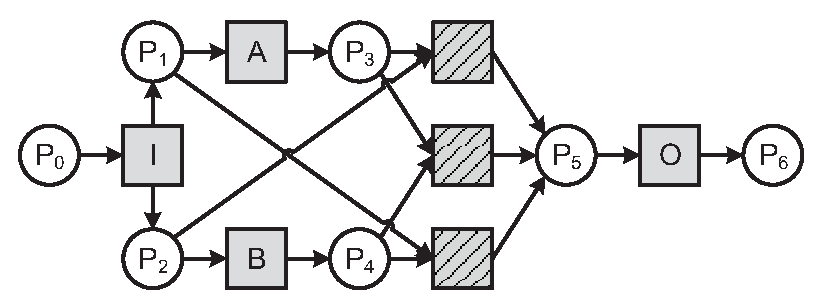
\includegraphics[width=0.9\textwidth]{fig_sda_example_1}
	\end{minipage}
	\label{fig:sdaExampleA}
}
\subfigure[] {
	\begin{minipage}[b]{0.45\textwidth}
		\centering
		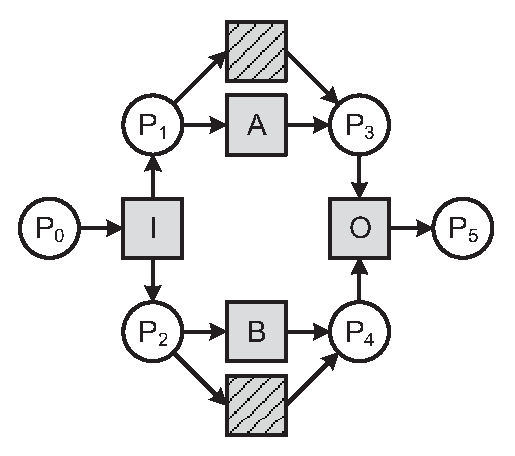
\includegraphics[width=0.9\textwidth]{fig_sda_example_2}
	\end{minipage}
	\label{fig:sdaExampleB}
}
\subfigure[] {
	\begin{minipage}[b]{0.45\textwidth}
		\centering
		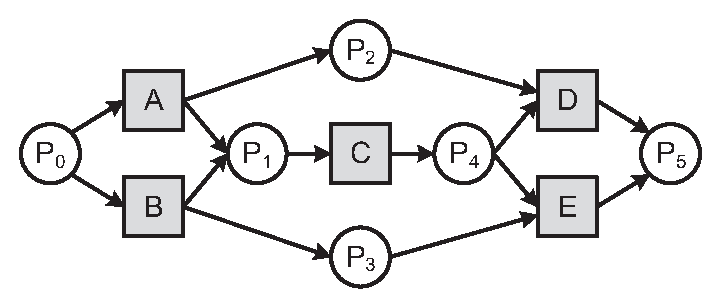
\includegraphics[width=0.9\textwidth]{fig_nfc_example_1}
	\end{minipage}
	\label{fig:nfcExampleA}
}
\subfigure[] {
	\begin{minipage}[b]{0.45\textwidth}
		\centering
		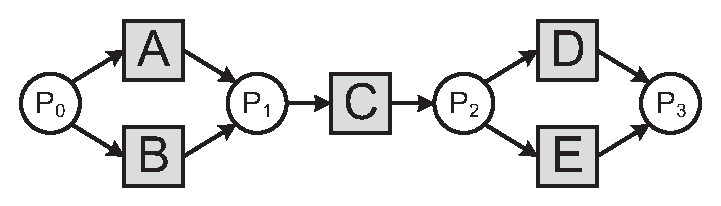
\includegraphics[width=0.9\textwidth]{fig_nfc_example_2}
	\end{minipage}
	\label{fig:nfcExampleB}
}
\caption{Examples where the work of Jin et al. fails to differentiate process models\label{fig:drawbacks}}
\end{figure}

In particular, the algorithm in \cite{jin2014computing} cannot work with cyclic WF-nets, which could be seen directly from the paper title. Furthermore, silent transitions have not been taken into consideration in \cite{jin2014computing} so that two WF-nets with different behavioral semantics may be regarded as the same. For example, the set of full firing sequences of the WF-net in Figure \ref{fig:sdaExampleA} is $\{\langle I,A,B,O\rangle$, $\langle I,B,A,O\rangle$, $\langle I,A,O\rangle$, $\langle I,B,O\rangle\}$, while the set of full firing sequences of the WF-net in Figure \ref{fig:sdaExampleB} is $\{\langle I,A,B,O\rangle$, $\langle I,B,A,O\rangle$, $\langle I,A,O\rangle$, $\langle I,B,O\rangle$, $\langle I,O\rangle\}$. Obviously, the behaviors of the two WF-nets in Figure~\ref{fig:sdaExampleA} and \ref{fig:sdaExampleB} are not the same. But the approach in \cite{jin2014computing} cannot distinguish them from each other.

In a WF-net with non-free-choice constructs \cite{de2003workflow}, sequential relations do not necessarily satisfy transitivity. Take the models in Figure \ref{fig:nfcExampleA} and \ref{fig:nfcExampleB} for example, we can capture the causal relations between $A$ and $C$ as well as $C$ and $E$ from both models. According to \cite{jin2014computing}, it can be inferred that $A$ and $E$ satisfy the causal relation. However, this is not correct in the WF-net with a non-free-choice construct in Figure \ref{fig:nfcExampleA} because only $C$ and $D$ can be executed if $A$ has been executed in the first place.

To solve these three major problems, we extend the ordering relations in \cite{jin2014computing} in a more fine-grained manner to uniquely differentiate the behavioral semantics of two process models. In addition to the idea of uncertainty, we also introduce the notion of multiple relations between a pair of tasks to reflect the fact that two tasks may have more than one relation between them.  This can allow us to capture subtle differences between any two processes.

A fine-grained characterization of all the relations among all pairs of tasks in a process model can serve as the basis of a proper similarity measure between process models. Other proposals have also addressed the problem of finding a suitable similarity measure between processes based on textual information, the topologies of process models, or their execution semantics \cite{weidlich2011efficient}. We give a quick introduction to some of them.

Zha et al. \cite{zha2010workflow} represent a process model's behavior by transition adjacency relations (TAR for short). But TAR cannot tackle the long-distance dependences between transitions, thus it is not able to handle specific structures like non-free-choice constructs. The BP algorithm \cite{weidlich2011efficient} represents the behavioral semantics of a process model based on behavioral profiles between transitions, but it cannot deal with silent transitions and distinguish parallel structures from loop structures. The PTS algorithm by Wang et al. \cite{wang2010behavioral} and its improvement CFS by Dong et al. \cite{dong2014cfs} utilize refined trace sets of process models to compute their similarity and are the most realistic results so far. But extracting the trace sets by both their methods is very time-consuming. Polyvyanyy et al. \cite{polyvyanyy20144c} propose a complete and fundamental notion of relations named 4C spectrum, which defines a repertoire of eighteen basic behavioral relations that capture such behavioral phenomena as co-occurrence, conflict, causality and concurrency \cite{armas2014suitability}, but \cite{polyvyanyy20144c} only gives the computation of four relations. Moreover, there exist two models that have the same 4C relations but induce differenct behavioral semantics \cite{armas2014suitability}, such as the two WF-nets in Figure \ref{fig:sdaExampleA} and \ref{fig:sdaExampleB}. Yan et al. \cite{yan2014efficient} decompose process models into small fragments, or features, based on which they analyze execution semantics to detect the differences between process models. However, their work lacks a global representation of the behavioral semantics of a model and only focuses on the local differences between two process models. Armas-Cervantes et al. \cite{armas2014behavioral} use asymmetric event structures (i.e., AES) to characterize the behaviors of process models and AES is more suitable to be utilized to compute the differences between two models.

There are three main contributions of this paper. First, it proposes a method called ExRORU that allows us to characterize all types of sound process models including those with cycles, silent transitions and non-free-choice constructs. Second, we argue informally that using ExRORU, we can detect behavioral differences between any pair of process models uniquely. Finally, we implement ExRORU and compare it with other algorithms that are also based on computing relations between transitions.

The remainder of this paper is structured as follows. The next section gives preliminaries that will be used throughout the paper. The concept and computation of ExRORU are introduced in Section \ref{sec:relations}. Section \ref{sec:experiments} shows the results of the experimental evaluation, before we conclude the paper and give an outlook on the future work in Section \ref{sec:conclusion}.

\section{Preliminaries}\label{sec:preliminaries}
We will show our algorithm on Petri nets. Other process models that could be converted to Petri nets are also applicable. The concept of Petri net has its origin in Carl Adam Petri's dissertation \cite{petri1966kommunikation}.

\begin{definition}[Petri net]\label{def:petrinet}
A Petri net is a triple $(P,T,F)$, where $P$ is a finite set of places, $T$ is a finite set of transitions ($P\cap T=\emptyset$ and $P\cup T=\emptyset$), and $F\subseteq(P\times T)\cup(T\times P)$ is a set of arcs (i.e., flow relation).
\end{definition}

We use $M:P\rightarrow\mathbb{N}$ to denote a marking of Petri net $N$, where $\mathbb{N}$ is the set of natural numbers. A Petri net system is a pair $\Sigma=(N,M_{0})$, where $N$ is a Petri net and $M_{0}$ is the initial marking of $N$. For more details about Petri net, please refer to the work of Murata \cite{murata1989petri}. A Petri net that models a workflow is called a Workflow net (i.e., WF-net) \cite{van1998application}.

\begin{definition}[WF-net]\label{def:wfnet}
A Petri net $PN=(P,T,F)$ is a WF-net if and only if $PN$ has two special places: $i$ and $o$, where place $i$ is a source place ($\bullet i=\emptyset$) and place $o$ is a sink place ($o\bullet =\emptyset$). If we add a transition $\overline{t}$ to $PN$ which connects place $o$ with $i$ (i.e. $\bullet \overline{t}=\{o\}$ and $\overline{t}\bullet=\{i\}$), then the resulting Petri net is strongly connected.
\end{definition}

According to \cite{esparza2002improvement}, there are three kinds of relations between nodes of a net.

\begin{definition}[Ordering Relations]\label{def:orderingRelations}
There are three types of ordering relations between any pair of nodes of a Petri net,
	\begin{itemize}
		\item[-] two nodes $x$ and $y$ are in causal relation, denoted by $x<y$, if the net contains a path with at least one arc leading from $x$ to $y$;
		\item[-] $x$ and $y$ are in conflict relation, denoted by $x\#y$, if the net contains two paths $st_{1}...x$ and $st_{2}...y$ starting at the same place $s$, and such that $t_{1}...x$ and $t_{2}...y$ are two disjoint paths;
		\item[-] $x$ and $y$ are in concurrency relation, denoted by $x~co~y$, if neither $x<y$ nor $y<x$ nor $x\#y$.
	\end{itemize}
\end{definition}

The full firing sequences, or execution sequences are suitable to capture some ordering relations between transitions. We introduce the notion of \textit{processes}, which can be utilized to represent \textit{causal} and \textit{concurrency} relation.

\begin{definition}[Causal net, adapted from \cite{polyvyanyy20144c}]\label{def:causalNet}
A net $N=(B,E,G)$ is a $causal~net$ iff: (i) for every $b\in B$ it holds that $|\bullet b|\leq 1$ and $|b\bullet|\leq 1$, and (ii) $N$ is acyclic.
\end{definition}

\begin{definition}[Process, adapted from \cite{polyvyanyy20144c}]\label{Process}
A $process$ of a system $S=(N,M)$, $N=(P,T,F)$, is an ordered pair $\pi=(N_{\pi},\rho)$, where $N_{\pi}=(B,E,G)$ is a causal net and $\rho:B\cup E\rightarrow P\cup T$ is a mapping function such that:
	\begin{itemize}
		\item[-] $\rho(B)\subseteq P$ and $\rho(E)\subseteq T$;
		\item[-] $Min(N_{\pi})$ is a cut and $\forall p\in P:M(p)=|\rho^{-1}(p)\cap Min(N_{\pi})|$, where a $cut$ of a causal net is a maximal (with respect to set inclusion) set of its pairwise concurrent conditions.
		\item[-] for every event $e\in E$ and for every place $p\in P$ it holds that $\bm{1}_{F}((p,\rho(e)))=|\rho^{-1}(p)\cap\bullet e|$ and $\bm{1}_{F}((\rho(e),p))=|\rho^{-1}(p)\cap e\bullet|$.\footnote{$\bm{1}_{F}$ denotes the characteristic function of $F$ on the set $(P\times T)\cup(T\times P)$.}
	\end{itemize}
\end{definition}

We can treat \textit{processes} as runs of a model, in which only causality and concurrency are explicitly captured. There are only sequential and parallel structures but neither loop nor exclusive structures in a process. In the next section, we will define our extended relations using the notion of \textit{processes}.

However, a Petri net system may have infinite processes due to the existence of loop structures, which differ on ``how much it unfolds''. It is not applicable to use the infinite processes to capture all the relations between transitions. Another intuitive idea is to generate the reachability graph of a WF-net, which has to face the problem of state space explosion \cite{mcmillan1995technique}. Javier Esparza et al. proposed the notion of complete prefix unfolding (CPU for short) to avoid this \cite{esparza2002improvement}. Therefore, we use his work instead.
% \begin{definition}[Occurrence net]\label{def:occurrenceNet}
% An occurrence net is a Petri net $O=(B,E,A)$ such that: $|\bullet b|\leq 1$ for every $b\in B$; $O$ is acyclic; $O$ is finitely preceded; no element is in conflict with itself.
% \end{definition}

% \begin{definition}[Branching process]\label{def:branchingProcess}
% A branching process of a Petri net system $\Sigma=(P,T,F,M_{0})$ is a labelled occurrence net $\beta=(B,E,A,f)$ where the labeling function $f$ satisfies the following properties:
% 	\begin{itemize}
% 		\item[-] $f(B)\subseteq P$ and $f(E)\subseteq T$ ($f$ preserves the nature of nodes);
% 		\item[-] for every $e\in E$, the restriction of $f$ to $\bullet e$ is a bijection between $\bullet e$ (in $\beta$) and $\bullet f(e)$ (in $\Sigma$), and similarly for $e\bullet$ and $f(e)\bullet$ ($f$ preserves the environments of transitions);
% 		\item[-] the restriction of $f$ to $Min(O)$ is a bijection between $Min(O)$ and $M_{0}$ ($\beta$ ``starts'' at $M_{0}$), where $Min(O)$ denotes the set of minimal elements of $B\cup E$ with respect to the causal relation;
% 		\item[-] for every $e_{1},e_{2}\in E$, if $\bullet e_{1}=\bullet e_{2}$ and $f(e_{1})=f(e_{2})$ then $e_{1}=e_{2}$ ($\beta$ does not duplicate the transitions of $\Sigma$).
% 	\end{itemize}
% \end{definition}

\begin{definition}[Complete Prefix Unfolding]\label{def:cpu}
Let $O=(B,E,A,f)$ be an occurrence net and $e\in E$ be any event.
	\begin{itemize}
		\item[-] A local configuration $\lceil e\rceil$ of an event $e$ in an occurrence net is the set of events that precede $e$.
		\item[-] The final marking of a local configuration $Mark(\lceil e\rceil)$ is the set of conditions that are marked after all the events in $\lceil e\rceil$ fire.
		\item[-] An adequate order $\prec$ is a strict well-founded partial order on local configurations, so that $\lceil e\rceil\subset\lceil e'\rceil$ implies $\lceil e\rceil\prec\lceil e'\rceil$\footnote{We use the definition of \emph{total order} for 1-safe systems defined in \cite{esparza2002improvement}.}.
		\item[-] An event $e$ of a branching process is a cutoff event if there exists a corresponding event $e'$, such that $Mark(\lceil e\rceil)=Mark(\lceil e'\rceil)$ and $\lceil e'\rceil\prec\lceil e\rceil$.
		\item[-] A complete prefix unfolding is the greatest backward closed subnet of an occurrence net containing no events after cutoff events.
	\end{itemize}
\end{definition}

Due to space limitation, we omit the explanations of CPU and related concepts such as \textit{occurrence net} and \textit{branching process}, which can be found in the work of Esparza \cite{esparza2002improvement} and Polyvyanyy \cite{polyvyanyy2010structuring}. Obviously, we can generate the set of processes of a WF-net from its CPU by ``unfolding'' the net after the cut-off events. In other words, CPU is the minimal but complete expression of all the runs in a model.

\begin{figure}[htbp]
\centering
\subfigure[A sound WF-net] {
	\centering
	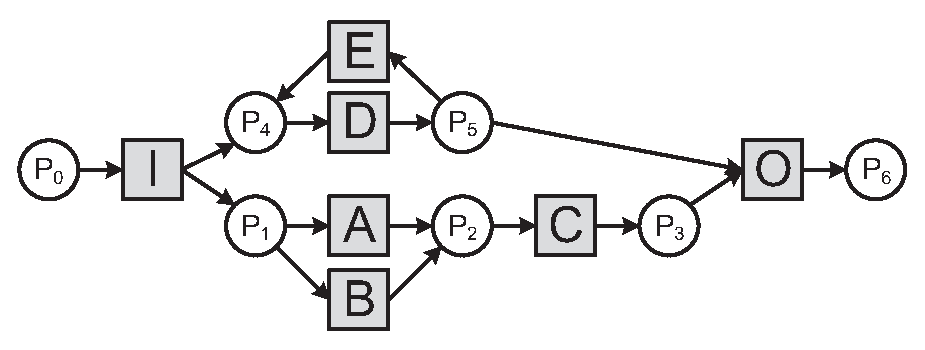
\includegraphics[width=0.45\textwidth]{fig_example_petri}
	\label{fig:examplePetri}
}
\subfigure[The CPU of \subref{fig:examplePetri}] {
	\centering
	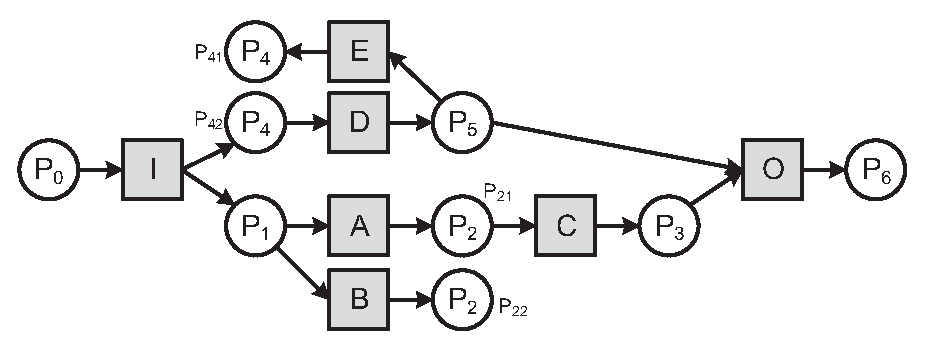
\includegraphics[width=0.45\textwidth]{fig_example_cpu}
	\label{fig:exampleCpu}
}
\caption{A sound WF-net example and its CPU\label{fig:examplePetriAndCpu}}
\end{figure}

\begin{example}\label{ex:petriAndCpu}
Figure \ref{fig:examplePetriAndCpu} shows a sound WF-net and its CPU. In the unfolding, events labelled as $B$ and $E$ are cutoff events. For event $B$, $A$ is its corresponding event while event $E$'s corresponding event is $I$.
\end{example}

% Our extended relations are inspired by the work in \cite{van2006decserflow}, which utilizes the relations between activities to model a process.
% \begin{definition}[Relation Formulas]\label{def:relationFormulas}
% Let $A$ and $B$ be two activities of a process, $A$ and $B$ are in the following relation formulas\footnote{The relation formulas \cite{van2006decserflow} are not complete here, since we only need part of them.}:
% 	\begin{itemize}
% 		\item[-] Response: when $A$ executes, $B$ has to be executed after it.
% 		\item[-] Precedence: $B$ could not have been executed until $A$ was executed.
% 		\item[-] Alternate Response: after the execution of $A$, $B$ has to be executed and between each two $A$ at least one $B$ has to be executed.
% 		\item[-] Alternate Precedence: before the execution of $B$, $A$ has to be executed first and between each two $B$ at least one $A$ has to be executed.
% 	\end{itemize}
% \end{definition}

% \begin{example}\label{ex:relationFormulas}
% In the WF-net of Figure \ref{fig:examplePetri}, $D,E$ in the execution sequence $\langle I,D,E,$\\$A,D,C,E,D,O\rangle$ satisfy the formula \textit{alternate response} and \textit{alternate precedence} while transitions $D,O$ do not satisfy the formula \textit{alternate response} and transitions $I,D$ do not satisfy the formula \textit{alternate precedence}.
% \end{example}

\section{Extended Refined Ordering Relations with Uncertainty}\label{sec:relations}
In this section, we introduce the concept of ExRORU and its calculation from a WF-net. Let $\Sigma=(P,T,F,M_{0})$ be a sound WF-net, and $U=(B,E,A,f)$ be its CPU. Let $x,y\in E$ be two events of the unfolding $U$.

\subsection{Extended Refined Causal Relations with Uncertainty}\label{subsec:causalAndInverseCausal}
CPU uses the technique of cutoff events to avoid the problem of state space explosion. We can set a mapping between cutoff conditions (conditions after cutoff events) and the conditions after the corresponding event of a cutoff event. Therefore, the processes generated from a CPU never ends on a cutoff condition, but will continue from the mapping of a cutoff condition instead.

We use expressions like $[ab\{c,d\}e]$ to represent the semantics of a process. Successive letters denote the sequential structure while letters in a brace mean a parallel structure. Different branches of a parallel structure are separated by a comma and could be nested. For example, in the CPU of Figure \ref{fig:exampleCpu}, $[I\{D,AC\}O]$, $[I\{D,BC\}O]$ and $[I\{DED,AC\}O]$ are some processes.

A trace, or execution sequence is a finite sequence of events $\sigma\in E^{*}$, leading from the source state to the end state by executing the events in order. Let $\Omega$ be the set containing all the traces of processes in $U$. Silent events are meaningless events for routing purpose only in models, which are not expresses in the control logic. We use shadowed box with slash to represent silent events, as shown in Figure \ref{fig:sdaExampleA} and \ref{fig:sdaExampleB}. Then we give the definition of \textit{Direct and Indirect Causal} relations based on whether two events can be executed adjacently in a trace.

\begin{definition}[Direct and Indirect Causal Relations]\label{def:sda}
Events $x$ and $y$ are in direct causal relation iff:
	\begin{itemize}
		\item[-] $x<y$;
		\item[-] $\exists\sigma=\langle t_{1},t_{2},...,t_{n}\rangle\in\Omega,1\leq i<j\leq n,t_{i}=x,t_{j}=y,s.t.~\forall k\in(i,j),t_{k}$ is a silent event.
	\end{itemize}
	% $x\overset{D}{\twoheadrightarrow}y$ or $x\overset{D}{\rightharpoonup}y$ (``D'' for direct) if they are in direct causal relation while $x\overset{I}{\twoheadrightarrow}y$ or $x\overset{I}{\rightharpoonup}y$ (``I'' for indirect) if not.
\end{definition}

Let $\Theta$ be the set containing all the processes generated from $U$, $\Theta_{x}$ be the set of the processes containing event $x$, i.e, $\Theta_{x}=\{\beta\in\Theta|x\in\beta\}$ and $FS(\beta)$ be the set of all the execution sequences of process $\beta$. Our extended causal relations are defined using the notion of $\Theta_{x}$ and $FS$.

\begin{definition}[Extended Causal Relations]\label{def:extendedCausal}
Events $x$ and $y$ are in:
	\begin{itemize}
		\item[-] always causal relation (denoted as $x\twoheadrightarrow y$) iff: $x<y$ and $\forall\beta_{x}\in\Theta_{x}$, $\forall\sigma\in FS(\beta_{x})$: after the execution of $x$, $y$ has to be executed and between each two $x$ (if there are more than one $x$) at least one $y$ has to be executed.
		\item[-] never causal relation (denoted as $x\nrightarrow y$) iff: $\forall\beta_{x}\in\Theta_{x}$, $\forall\sigma\in FS(\beta_{x})$: when $x$ executes, $y$ mustn't be executed after it.
		\item[-] sometimes causal relation (denoted as $x\rightharpoonup y$) iff: neither $x\twoheadrightarrow y$ nor $x\nrightarrow y$.
	\end{itemize}
	Further, $x\overset{D}{\twoheadrightarrow}y$ or $x\overset{D}{\rightharpoonup}y$ (``D'' for direct) if they are in direct causal relation while $x\overset{I}{\twoheadrightarrow}y$ or $x\overset{I}{\rightharpoonup}y$ (``I'' for indirect) if not.
\end{definition}

The relations above are collectively called extended refined causal relation with uncertainty (denoted as $\rightarrow$).

\begin{example}\label{ex:causalRelation}
In the CPU of Figure \ref{fig:exampleCpu}, $A$ and $C$ are in \textit{direct always causal} relation (i.e., $A\overset{D}{\twoheadrightarrow}C$) since they satisfy the conditions among all the traces containing $A$ and they can be executed adjacently. $E$ and $O$ are in \textit{indirect sometimes causal} relation (i.e., $E\overset{I}{\rightharpoonup}O$) since there may be another $E$ between the first $E$ and $O$, and there must be at least one $D$ between them. $A$ and $B$ are in \textit{never causal} relation (i.e., $A\nrightarrow B$).
\end{example}

\textbf{Always Inverse Causal} ($\twoheadleftarrow$), \textbf{Sometimes Inverse Causal} ($\leftharpoonup$) and \textbf{Never Inverse Causal} ($\nleftarrow$) can be defined in a similar way. The relations above are collectively called extended refined inverse causal relation with uncertainty (denoted as $\leftarrow$). Also, we further refine $\twoheadleftarrow$ and $\leftharpoonup$ into four relations, i.e., $\overset{D}{\twoheadleftarrow}$, $\overset{I}{\twoheadleftarrow}$, $\overset{D}{\leftharpoonup}$ and $\overset{I}{\leftharpoonup}$.

% \begin{definition}[Always Inverse Causal]\label{def:alwaysInverseCausal}
% Events $y$ and $x$ are in always inverse causal relation (denoted as $y\twoheadleftarrow x$) iff: $\forall\beta_{y}\in\Theta_{y}$, $x$ and $y$ are in \textit{alternate precedence} relation, i.e., among all the branching processes containing event $y$, every instance of $y$ has to be preceded by an instance of $x$ and the next instance of event $y$ cannot be executed before the next instance of event $x$ is executed.
% \end{definition}

% \begin{definition}[Never Inverse Causal]\label{def:neverInverseCausal}
% Events $y$ and $x$ are in never inverse causal relation (denoted as $y\nleftarrow x$) iff: $\forall\beta_{y}\in\Theta_{y}$, $x$ and $y$ are not in \textit{precedence} relation, i.e., among all the branching processes containing event $y$, before the execution of every $y$, there mustn't be an instance of $a$ executed.
% \end{definition}

% \begin{definition}[Sometimes Inverse Causal]\label{def:sometimesInverseCausal}
% Events $y$ and $x$ are in sometimes inverse causal relation (denoted as $y\leftharpoonup x$) iff: neither $y\twoheadleftarrow x$ nor $y\nleftarrow x$.
% \end{definition}

\begin{example}
In the CPU of Figure \ref{fig:exampleCpu}, $O$ and $D$ are in \textit{direct always inverse causal} relation (i.e., $O\overset{D}{\twoheadleftarrow}D$) since they satisfy the conditions among all the traces containing $O$ and they can be executed adjacently. $O$ and $A$ are in \textit{indirect sometimes inverse causal} relation (i.e., $O\overset{I}{\leftharpoonup}A$) since there may be no instance of event $A$ in some traces containing $O$ and there must be an event $C$ in front of $O$. $A$ and $B$ are in \textit{never inverse causal} relation (i.e., $A\nleftarrow B$).
\end{example}

We have identified several cases of causal and inverse causal relations and turned them into abstract formulas as shown in Figure \ref{fig:causalCases}. We use part of the unfolding instead of the massive processes to save space. In these cases, $A$ and $B$ are events of an unfolding. The edge labeled with ``Loop $X$'' means that there is a path starting from some condition after $X$ and ending in some condition before $X$ so that $X$ can be executed more than once. The edge labeled with ``Skip $X$'' means that there is a path starting from some condition before $X$ and ending in some condition after $X$ so that $X$ may not be executed. %In other words, events inside a \textit{loop} structure can be executed more than once while events inside a \textit{skip} structure may not be executed.

\begin{figure}[htbp]
\centering
\subfigure[] {
	\begin{minipage}[b]{0.45\textwidth}
		\centering
		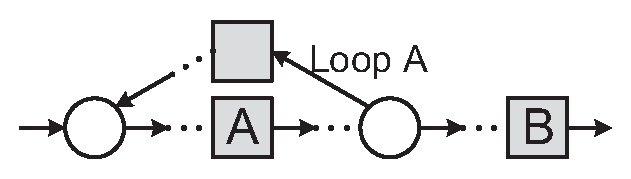
\includegraphics[width=0.8\textwidth]{fig_causal_case_a_1}\\
		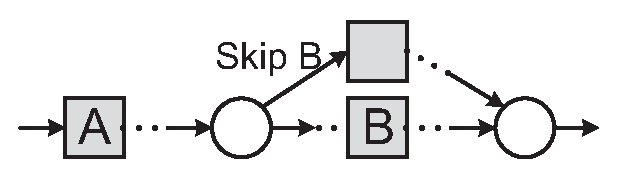
\includegraphics[width=0.8\textwidth]{fig_causal_case_a_2}
	\end{minipage}
	\label{fig:causalCaseA}
}
\subfigure[] {
	\begin{minipage}[b]{0.45\textwidth}
		\centering
		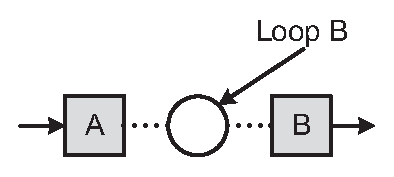
\includegraphics[width=0.8\textwidth]{fig_causal_case_b_1}
		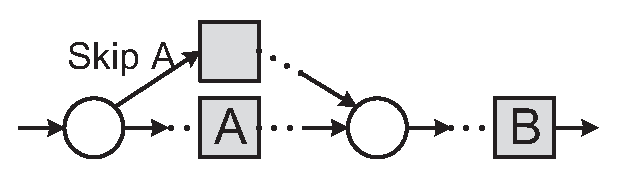
\includegraphics[width=0.8\textwidth]{fig_causal_case_b_2}
	\end{minipage}
	\label{fig:causalCaseB}
}
\subfigure[] {
	\begin{minipage}[b]{0.45\textwidth}
		\centering
		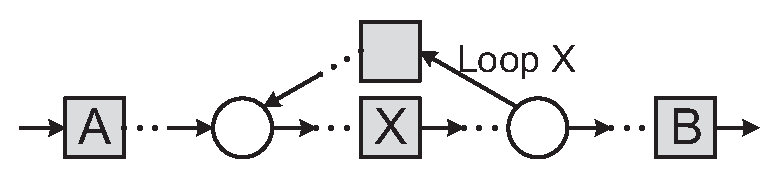
\includegraphics[width=1.0\textwidth]{fig_causal_case_c}
	\end{minipage}
	\label{fig:causalCaseC}
}
\subfigure[] {
	\begin{minipage}[b]{0.45\textwidth}
		\centering
		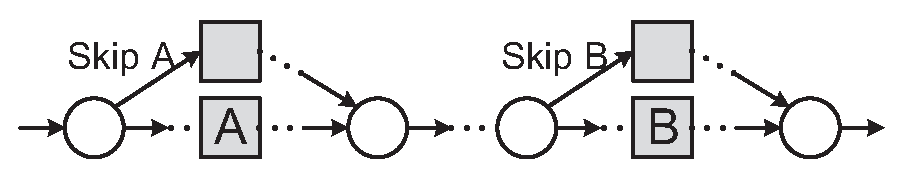
\includegraphics[width=1.0\textwidth]{fig_causal_case_d}
	\end{minipage}
	\label{fig:causalCaseD}
}
\caption{Abstract formulas of causal and inverse causal relations. \subref{fig:causalCaseA} $A\rightharpoonup B, B\twoheadleftarrow A$; \subref{fig:causalCaseB} $A\twoheadrightarrow B, B\leftharpoonup A$; \subref{fig:causalCaseC} $A\twoheadrightarrow B, B\twoheadleftarrow A$; \subref{fig:causalCaseD} $A\rightharpoonup B, B\leftharpoonup A$.\label{fig:causalCases}}
\end{figure}

% \textcolor{red}{Compress the following two paragraphs}
We omit the \textit{direct} and \textit{indirect} symbol since we cannot determine them in these abstract formulas. For convenience, we use symbol $*$ to represent any numbers of sequential events excluding $A$ and $B$. In Figure \ref{fig:causalCaseA}, we have processes such as $[A*B],[A*A*B],[A*A*A*B]$ for the upper unfolding and $[A*B],[A*]$ for the lower unfolding, both of which indicate that $A$ and $B$ are in \textit{sometimes causal} relation and \textit{always inverse causal} relation, i.e., $A\rightharpoonup B,B\twoheadleftarrow A$. Similarly in Figure \ref{fig:causalCaseB}, we have $A\twoheadrightarrow B,B\leftharpoonup A$.

In Figure \ref{fig:causalCaseC}, a loop structure in the middle part of an unfolding will certainly not affect the extended relations between $A$ and $B$, neither will an exclusive structure, i.e., $A\twoheadrightarrow B,B\twoheadleftarrow A$. However, if there are exclusive structures across both $A$ and $B$, such as the unfolding in Figure \ref{fig:causalCaseD}, which has processes such as $[A*B],[A*],[*B],[*]$, then $A\rightharpoonup B$ and $B\leftharpoonup A$.

\subsection{Extended Refined Concurrent Relations with Uncertainty}\label{subsec:concurrent}
We use $\Omega_{x}$ to denote the set of the traces containing event $x$, i.e., $\Omega_{x}=\{\sigma\in\Omega|x\in\sigma\}$. Our extended concurrent relations are defined using the notion of $\Omega_{x}$.

We use $\sigma\uparrow X$ to denote the projection of $\sigma$ onto some event set $X\subseteq E$, i.e., a trace $\sigma'\subseteq\sigma$ which only contains those events in $X$ and remains their order in $\sigma$. Let $P(\sigma,x,y)=\sigma\uparrow\{x,y\}$ be the projection of $\sigma$ onto events $x$ and $y$.

\begin{definition}[Extended Concurrent Relations]\label{def:extendedConcurrent}
Events $x$ and $y$ are in:
	\begin{itemize}
		\item[-] always concurrent relation (denoted as $x\Updownarrow y$) iff: $\forall\sigma_{x}\in\Omega_{x}$, $x~co~y$ and $(|P|\%2=0\vee(|P|\%2=1\wedge P_{|P|}=y))\wedge\forall_{0\leq k<|P|/2}((P_{2k+1}=x\wedge P_{2k+2}=y)\vee(P_{2k+1}=y\wedge P_{2k+2}=x)\vee(P_{2k+1}=y\wedge P_{2k+2}=y))$, where $P$ is the abbreviation of $P(\sigma_{x},x,y)$;
		\item[-] never concurrent relation (denoted as $x\nparallel y$) iff: $\forall\sigma_{x}\in\Omega_{x}$, $x$ and $y$ are not in concurrency relation;
		\item[-] sometimes concurrent relation (denoted as $x\Uparrow y$) iff: neither $x\Updownarrow y$ nor $x\nparallel y$.
	\end{itemize}
\end{definition}

The relations above are collectively called extended refined concurrent relations with uncertainty (denoted as $\parallel$). We have also identified several cases of concurrent relations and turn them into abstract formulas, as shown in Figure \ref{fig:concurrentCases}.

\begin{figure}[htbp]
\centering
\subfigure[] {
	\begin{minipage}[b]{1\textwidth}
		\centering
		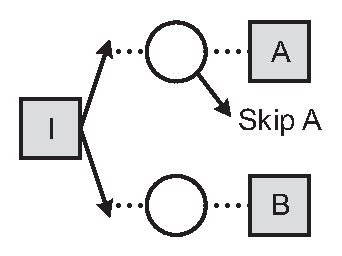
\includegraphics[width=0.3\textwidth]{fig_concurrent_case_a_1}
		\hspace{0.5in}
		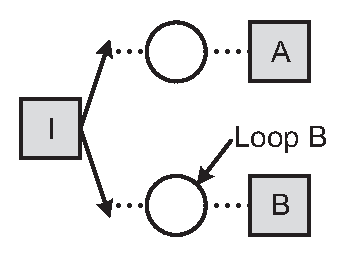
\includegraphics[width=0.3\textwidth]{fig_concurrent_case_a_2}
	\end{minipage}
	\label{fig:concurrentCaseA}
}
\subfigure[] {
	\begin{minipage}[b]{0.3\textwidth}
		\centering
		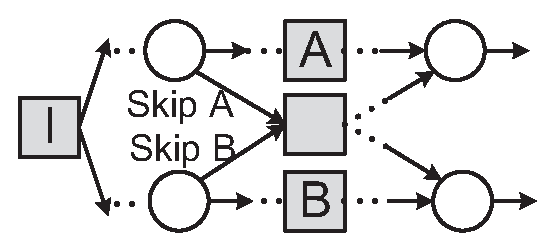
\includegraphics[width=1.0\textwidth]{fig_concurrent_case_b}
	\end{minipage}
	\label{fig:concurrentCaseB}
}
\subfigure[] {
	\begin{minipage}[b]{0.3\textwidth}
		\centering
		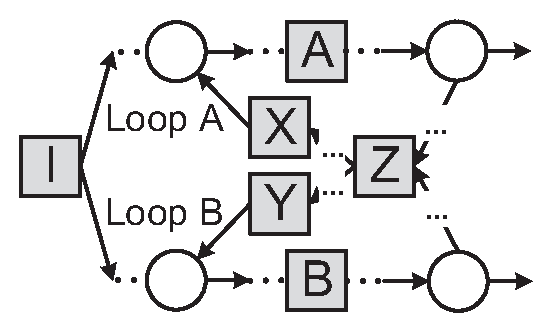
\includegraphics[width=1.0\textwidth]{fig_concurrent_case_c}
	\end{minipage}
	\label{fig:concurrentCaseC}
}
\subfigure[] {
	\begin{minipage}[b]{0.3\textwidth}
		\centering
		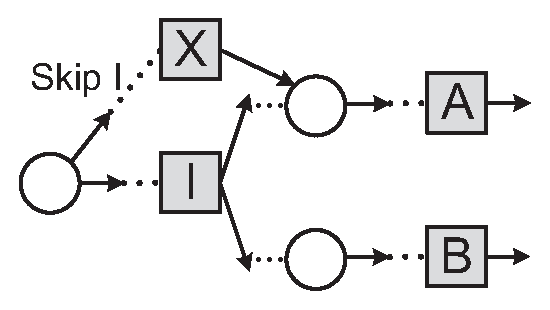
\includegraphics[width=1.0\textwidth]{fig_concurrent_case_d}
	\end{minipage}
	\label{fig:concurrentCaseD}
}
\caption{Abstract formulas of concurrent relations. \subref{fig:concurrentCaseA} $A\Uparrow B,B\Updownarrow A$; \subref{fig:concurrentCaseB} $A\Updownarrow B,B\Updownarrow A$; \subref{fig:concurrentCaseC} $A\Updownarrow B,B\Updownarrow A$; \subref{fig:concurrentCaseD} $A\Uparrow B,B\Updownarrow A$.\label{fig:concurrentCases}}
\end{figure}

In Figure \ref{fig:concurrentCaseA}, we have traces such as $\langle I*A*B*\rangle ,\langle I*B*A*\rangle ,\langle I*A*\rangle $ for the left unfolding and traces such as $\langle I*A*B*\rangle ,\langle I*A*A*B*\rangle ,\langle I*A*A*A*B*\rangle$ for the right unfolding, which do not satisfy the conditions in Definition \ref{def:extendedConcurrent}. Therefore, events $A$ and $B$ are in \textit{sometimes concurrent} relation, i.e., $A\Uparrow B$. As for the unfolding in Figure \ref{fig:concurrentCaseB}, events $A$ and $B$ may be executed both once or not executed at all, indicating that $A\Updownarrow B$. It is easily seen that traces in the unfolding of Figure \ref{fig:concurrentCaseC} satisfy the conditions in Definition \ref{def:extendedConcurrent}, so $A$ and $B$ are in \textit{always concurrent} relation, i.e., $A\Updownarrow B$. The unfolding in Figure \ref{fig:concurrentCaseD} shows a non-free-choice construct, which we will go into details later.

Table \ref{tab:relations} shows the summary of all proposed relations for ExRORU.

\begin{table}[htbp]
\centering
\caption{Summary of all proposed relations for ExRORU\label{tab:relations}}
	\begin{tabular}{|c|l||c|l||c|l|} \hline
		& \multicolumn{1}{|c||}{\multirow{1}{*}{Description}} & & \multicolumn{1}{|c||}{\multirow{1}{*}{Description}} & & \multicolumn{1}{|c|}{\multirow{1}{*}{Description}}\\ \hline
		$\overset{D}{\twoheadrightarrow}$ & \textit{direct always causal} & $\overset{D}{\twoheadleftarrow}$ & \textit{direct always inverse causal} & $\Updownarrow$ & \textit{always concurrent}\\
		$\overset{I}{\twoheadrightarrow}$ & \textit{indirect always causal} & $\overset{I}{\twoheadleftarrow}$ & \textit{indirect always inverse causal} & $\Uparrow$ & \textit{sometimes concurrent}\\
		$\overset{D}{\rightharpoonup}$ & \textit{direct sometimes causal} & $\overset{D}{\leftharpoonup}$ & \textit{direct sometimes inverse causal} & $\nparallel$ & \textit{never concurrent}\\
		$\overset{I}{\rightharpoonup}$ & \textit{indirect sometimes causal} & $\overset{I}{\leftharpoonup}$ & \textit{indirect sometimes inverse causal} & & \\
		$\nrightarrow$ & \textit{never causal} & $\nleftarrow$ & \textit{never inverse causal} & & \\
		\hline
	\end{tabular}
\end{table}

\subsection{Computing ExRORUs from an Unfolding}\label{subsec:computationOfRelations}
%As mentioned before, an intuitive idea to derive our relations is based on reachability graphs. Such technique would face a state explosion problem, especially when the WF-net contains a parallel with large scale of transitions. Theoretically, the reachability graph will derive all the reachable states by combining the executions of transitions within a parallel structure. Another problem is that we actually cannot distinguish the causal relation caused by loop structure and parallel structure using the reachability technique. By definitions, causal relations caused by parallel structure are not considered in our extended refined ordering relations. 
As mentioned before, using reachability graphs to derive our relations would face the problem of state space explosion. %And we actually cannot distinguish the causal relation caused by loop and parallel structure using the reachability technique, the latter of which is not considered in our definitions. 
So we adopt the ``unfolding technology'' in this paper. It is also impossible to derive the relations based on a sound WF-net itself directly because a WF-net describes the structure of a process rather than its behavior.

Another intuitive idea is to check our causal relations based on all the processes, i.e., $\Theta$ of a CPU. However, $\Theta$ may be an infinite set, which is not practical to compute and utilize. Therefore, motivated by the abstract formulas in Figure \ref{fig:causalCases}, we will derive our relations on a CPU by tracing the directed path from one event to another and check every condition to determine whether there is a \textit{loop} or \textit{skip} structure.

Similarly, we can trace backwards along the path from one event to another to derive the inverse causal relations between them. It should be noticed that $\rightarrow$ and $\leftarrow$ may not have the same uncertainty for one pair of events. For example, we have $A\overset{I}{\twoheadrightarrow}O$ but $O\overset{I}{\leftharpoonup}A$ in the CPU of Figure \ref{fig:exampleCpu}. Furthermore, $D\overset{D}{\rightharpoonup}E$ and $E\overset{D}{\twoheadrightarrow}D$ both exist due to the cycle in the CPU, which cannot be computed in \cite{jin2014computing} at all.

As for the extended concurrent relations between events $a$ and $b$, there are actually two relations which should be taken into consideration, i.e., $a\parallel b$ and $b\parallel a$. We firstly find the entrance of the parallel structure, and trace the path from it to $a$ and $b$. As Figure \ref{fig:concurrentCases} shows, by checking every condition to find out all the \textit{loop} and \textit{skip} structures, we can derive the extended concurrent relations between them.

Now we have defined the relations between events in a CPU, which will be utilized to compute the relations between transitions in a WF-net next. In general, there may be more than one corresponding event in the CPU related to a transition in the original WF-net. These corresponding events are different from each other and are treated as unique events when we derive the relations between events in the unfolding. Therefore, when we try to derive the ExRORUs between transitions in the WF-net, we need to check the relations between each pair of corresponding events of those transitions. Based on this, we give the computation of ExRORU between transitions. Let $Corr_{E}(A)$ be the set containing all the corresponding events of transition $A$.

\begin{definition}[Extended Causal Relations Between Transitions]\label{def:causalRelations}
Transitions $A$ and $B$ are in: 
	\begin{itemize}
		\item[-] \textbf{always causal relation} (denoted as $A\twoheadrightarrow B$) iff: $\forall a\in Corr_{E}(A), \exists b\in Corr_{E}(B), s.t.~a\twoheadrightarrow b$. Further, $A\overset{D}{\twoheadrightarrow}B$ if $\exists a\in Corr_{E}(A), b\in Corr_{E}(B),$ $s.t.~a\overset{D}{\twoheadrightarrow}b$; $A\overset{I}{\twoheadrightarrow}B$ otherwise.
		\item[-] \textbf{never causal relation} (denoted as $A\nrightarrow B$) iff: $\forall a\in Corr_{E}(A), \forall b\in Corr_{E}(B), a\nrightarrow b$.
		\item[-] \textbf{sometimes causal relation} (denoted as $A\rightharpoonup B$) iff: neither $A\twoheadrightarrow B$ nor $A\nrightarrow B$. Further, $A\overset{D}{\rightharpoonup}B$ if $\exists a\in Corr_{E}(A), b\in Corr_{E}(B), s.t.~a\overset{D}{\rightharpoonup}b$; $A\overset{I}{\rightharpoonup}B$ otherwise.
	\end{itemize}  
\end{definition}

\begin{definition}[Extended Inverse Causal Relations Between Transitions]\label{def:inverseCausalRelations}
Transitions $B$ and $A$ are in: 
	\begin{itemize}
		\item[-] \textbf{always inverse causal relation} (denoted as $B\twoheadleftarrow A$) iff: $\forall b\in Corr_{E}(B), \exists a\in Corr_{E}(A), s.t.~b\twoheadleftarrow a$. Further, $B\overset{D}{\twoheadleftarrow}A$ if $\exists b\in Corr_{E}(B), a\in Corr_{E}(A),s.t.~b\overset{D}{\twoheadleftarrow}a$; $B\overset{I}{\twoheadleftarrow}A$ otherwise.
		\item[-] \textbf{never inverse causal relation} (denoted as $B\nleftarrow A$) iff: $\forall b\in Corr_{E}(B), \forall a\in Corr_{E}(A), b\nleftarrow a$.
		\item[-] \textbf{sometimes inverse causal relation} (denoted as $B\leftharpoonup A$) iff: neither $B\twoheadleftarrow A$ nor $B\nleftarrow A$. Further, $B\overset{D}{\leftharpoonup}A$ if $\exists b\in Corr_{E}(B), a\in Corr_{E}(A), s.t.~b\overset{D}{\leftharpoonup}a$; $B\overset{I}{\leftharpoonup}A$ otherwise.
	\end{itemize}
\end{definition}

\begin{definition}[Extended Concurrent Relations Between Transitions]\label{def:concurrentRelations}
Transitions $A$ and $B$ are in: 
	\begin{itemize}
		\item[-] \textbf{always concurrent relation} (denoted as $A\Updownarrow B$) iff: $\forall a\in Corr_{E}(A),\exists b\in Corr_{E}(B),s.t.~a\Updownarrow b$;
		\item[-] \textbf{never concurrent relation} (denoted as $A\nparallel B$) iff: $\forall a\in Corr_{E}(A),\forall b\in Corr_{E}(B),a\nparallel b$;
		\item[-] \textbf{sometimes concurrent relation} (denoted as $A\Uparrow B$) iff: neither $A\Updownarrow B$ nor $A\nparallel B$.
	\end{itemize}
\end{definition}

In general, using the notions and computations described in the previous sections, we can derive ExRORUs of any process model. The ExRORU for the model in Figure \ref{fig:examplePetri} is shown in Table \ref{tab:example_relations}. For convenience, we use three separate matrices to represent the three types of relations. Each ($X$,$Y$) entry in a matrix shows the relation between transitions $X$ and $Y$. Moreover, in general, multiple relations may exist between $X$ and $Y$ as we discuss in the next section.

\begin{table}[htbp]
\centering
\caption{Extended refined ordering relations of the WF-net in Figure \ref{fig:examplePetri}\label{tab:example_relations}}
\begin{tabular}{|c|c|c|c|c|c|c|c!{\vrule width 1.5pt}c|c|c|c|c|c|c|c!{\vrule width 1.5pt}c|c|c|c|c|c|c|c|} \hline
	$\rightarrow$ & $A$ & $B$ & $C$ & $D$ & $E$ & $I$ & $O$ & 
	$\leftarrow$ & $A$ & $B$ & $C$ & $D$ & $E$ & $I$ & $O$ & 
	$\parallel$ & $A$ & $B$ & $C$ & $D$ & $E$ & $I$ & $O$\\ \hline
	
	$A$ & $\nrightarrow$ & $\nrightarrow$ & $\overset{D}{\twoheadrightarrow}$ & $\nrightarrow$ & $\nrightarrow$ & $\nrightarrow$ & $\overset{I}{\twoheadrightarrow}$ &
	$A$ & $\nleftarrow$ & $\nleftarrow$ & $\nleftarrow$ & $\nleftarrow$ & $\nleftarrow$ & $\overset{D}{\twoheadleftarrow}$ & $\nleftarrow$ &
	$A$ & $\nparallel$ & $\nparallel$ & $\nparallel$ & $\Updownarrow$ & $\Uparrow$ & $\nparallel$ & $\nparallel$\\ \hline

	$B$ & $\nrightarrow$ & $\nrightarrow$ & $\overset{D}{\twoheadrightarrow}$ & $\nrightarrow$ & $\nrightarrow$ & $\nrightarrow$ & $\overset{I}{\twoheadrightarrow}$ &
	$B$ & $\nleftarrow$ & $\nleftarrow$ & $\nleftarrow$ & $\nleftarrow$ & $\nleftarrow$ & $\overset{D}{\twoheadleftarrow}$ & $\nleftarrow$ &
	$B$ & $\nparallel$ & $\nparallel$ & $\nparallel$ & $\Updownarrow$ & $\Uparrow$ & $\nparallel$ & $\nparallel$\\ \hline

	$C$ & $\nrightarrow$ & $\nrightarrow$ & $\nrightarrow$ & $\nrightarrow$ & $\nrightarrow$ & $\nrightarrow$ & $\overset{D}{\twoheadrightarrow}$ &
	$C$ & $\overset{D}{\leftharpoonup}$ & $\overset{D}{\leftharpoonup}$ & $\nleftarrow$ & $\nleftarrow$ & $\nleftarrow$ & $\overset{I}{\twoheadleftarrow}$ & $\nleftarrow$ &
	$C$ & $\nparallel$ & $\nparallel$ & $\nparallel$ & $\Updownarrow$ & $\Uparrow$ & $\nparallel$ & $\nparallel$\\ \hline

	$D$ & $\nrightarrow$ & $\nrightarrow$ & $\nrightarrow$ & $\overset{I}{\rightharpoonup}$ & $\overset{D}{\rightharpoonup}$ & $\nrightarrow$ & $\overset{D}{\rightharpoonup}$ &
	$D$ & $\nleftarrow$ & $\nleftarrow$ & $\nleftarrow$ & $\overset{I}{\leftharpoonup}$ & $\overset{D}{\leftharpoonup}$ & $\overset{D}{\leftharpoonup}$ & $\nleftarrow$ &
	$D$ & $\Uparrow$ & $\Uparrow$ & $\Uparrow$ & $\nparallel$ & $\nparallel$ & $\nparallel$ & $\nparallel$\\ \hline

	$E$ & $\nrightarrow$ & $\nrightarrow$ & $\nrightarrow$ & $\overset{D}{\twoheadrightarrow}$ & $\overset{I}{\rightharpoonup}$ & $\nrightarrow$ & $\overset{I}{\twoheadrightarrow}$ &
	$E$ & $\nleftarrow$ & $\nleftarrow$ & $\nleftarrow$ & $\overset{D}{\twoheadleftarrow}$ & $\overset{I}{\leftharpoonup}$ & $\overset{I}{\leftharpoonup}$ & $\nleftarrow$ &
	$E$ & $\Uparrow$ & $\Uparrow$ & $\Uparrow$ & $\nparallel$ & $\nparallel$ & $\nparallel$ & $\nparallel$\\ \hline

	$I$ & $\overset{D}{\rightharpoonup}$ & $\overset{D}{\rightharpoonup}$ & $\overset{I}{\twoheadrightarrow}$ & $\overset{D}{\twoheadrightarrow}$ & $\overset{I}{\rightharpoonup}$ & $\nrightarrow$ & $\overset{I}{\twoheadrightarrow}$ &
	$I$ & $\nleftarrow$ & $\nleftarrow$ & $\nleftarrow$ & $\nleftarrow$ & $\nleftarrow$ & $\nleftarrow$ & $\nleftarrow$ &
	$I$ & $\nparallel$ & $\nparallel$ & $\nparallel$ & $\nparallel$ & $\nparallel$ & $\nparallel$ & $\nparallel$\\ \hline

	$O$ & $\nrightarrow$ & $\nrightarrow$ & $\nrightarrow$ & $\nrightarrow$ & $\nrightarrow$ & $\nrightarrow$ & $\nrightarrow$ &
	$O$ & $\overset{I}{\leftharpoonup}$ & $\overset{I}{\leftharpoonup}$ & $\overset{D}{\twoheadleftarrow}$ & $\overset{D}{\twoheadleftarrow}$ & $\overset{I}{\leftharpoonup}$ & $\overset{I}{\twoheadleftarrow}$ & $\nleftarrow$ &
	$O$ & $\nparallel$ & $\nparallel$ & $\nparallel$ & $\nparallel$ & $\nparallel$ & $\nparallel$ & $\nparallel$\\ \hline
\end{tabular}
\end{table}

An extensive characterization of a process model in terms of various relations between every pair of transitions in it in this manner produces a \textit{unique fingerprint} for each model. A formal proof is outside the scope of our current work. An informal argument relies on the fact that given any process model, if we make any primitive change to it such as adding, deleting or restructuring a visible or silent transition the fingerprint for this model will always change. Thus, the difference between two models can always be detected.

% \subsection{Sequential Direct Adjacency between Transitions}\label{subsec:sda}
% We can distinguish most process models from each other by their executing semantics using ExRORU if silent transitions are not introduced. Silent transitions do not appear in any log trace but have effects on the behavior of a WF-net \cite{de2003workflow}.

% \begin{table}[htbp]
% \centering
% \tabcaption{ExRORUs of the two models in Figure \ref{fig:sdaExampleA} and \ref{fig:sdaExampleB}\label{tab:sdaExample}}
% \begin{tabular}{c|c|c|c|c} \hline
% 	Transitions & $A$ & $B$ & $I$ & $O$\\ \hline
% 	$A$
% 		& $\nrightarrow\nleftarrow\nparallel$
% 		& $\nrightarrow\nleftarrow\Uparrow$
% 		& $\nrightarrow\twoheadleftarrow\nparallel$
% 		& $\twoheadrightarrow\nleftarrow\nparallel$
% 		\\ \hline
% 	$B$
% 		& $\nrightarrow\nleftarrow\Uparrow$
% 		& $\nrightarrow\nleftarrow\nparallel$
% 		& $\nrightarrow\twoheadleftarrow\nparallel$
% 		& $\twoheadrightarrow\nleftarrow\nparallel$
% 		\\ \hline
% 	$I$
% 		& $\rightharpoonup\nleftarrow\nparallel$
% 		& $\rightharpoonup\nleftarrow\nparallel$
% 		& $\nrightarrow\nleftarrow\nparallel$
% 		& $\twoheadrightarrow\nleftarrow\nparallel$
% 		\\ \hline
% 	$O$
% 		& $\nrightarrow\leftharpoonup\nparallel$
% 		& $\nrightarrow\leftharpoonup\nparallel$
% 		& $\nrightarrow\twoheadleftarrow\nparallel$
% 		& $\nrightarrow\nleftarrow\nparallel$
% 		\\ \hline
% \end{tabular}
% \end{table}

% As shown in Table \ref{tab:sdaExample}, the ExRORUs of the two models in Figure \ref{fig:sdaExampleA} and \ref{fig:sdaExampleB} are the same, but the behavioral sementics of them are not (refer to Example \ref{ex:drawback2}). By looking into the executing semantics of these models, we find that the introduction of silent transitions influences the adjacency of visible transitions, i.e., $I$ can be directly followed by $O$ in Figure \ref{fig:sdaExampleB}, but not in Figure \ref{fig:sdaExampleA}. Inspired by the idea of TAR \cite{zha2010workflow}, we propose the concept of sequential direct adjacency to take the effects of silent transitions into consideration.

% \begin{definition}[Sequential Direct Adjacency]\label{def:sda}
% Let $\Sigma=(P,T,F,M_{0})$ be a WF-net and $A,B\in T$ are two visible transitions. $A$ and $B$ are in sequential direct adjacency iff:
% 	\begin{itemize}
% 		\item[-] $A$ and $B$ are not in cocurrency relation;
% 		\item[-] $\exists\sigma=\langle t_{1},t_{2},...,t_{n}\rangle\in\Omega,1\leq i<j\leq n,t_{i}=A,t_{j}=B,s.t.~\forall k\in(i,j),t_{k}$ is a silent transition.
% 	\end{itemize}
% $A\overset{D}{\rightarrow}B$ (``D" for \textit{direct}) if they are in sequential direct adjacency while $A\overset{I}{\rightarrow}B$ (``I" for \textit{indirect}) if not. Similarly, we can also define SDA on $\leftarrow$ relation, denoted as $B\overset{D}{\leftarrow}A$ and $B\overset{I}{\leftarrow}A$.
% \end{definition}

% We use SDA to distinguish those transition pairs which can be executed adjacently from those which cannot. By applying Definition \ref{def:sda} on the two models in Figure \ref{fig:sdaExampleA} and \ref{fig:sdaExampleB}, we derive further refined ExRORUs as follows:
% \begin{displaymath}
% 	\begin{aligned}
% 		\text{(a)} & A\overset{D}{\twoheadrightarrow}O, B\overset{D}{\twoheadrightarrow}O, I\overset{D}{\rightharpoonup}A, I\overset{D}{\rightharpoonup}B, I\overset{I}{\twoheadrightarrow}O\\
% 		& O\overset{D}{\leftharpoonup}A, O\overset{D}{\leftharpoonup}B, A\overset{D}{\twoheadleftarrow}I, B\overset{D}{\twoheadleftarrow}I, O\overset{I}{\twoheadleftarrow}I\\
% 		\text{(b)} & A\overset{D}{\twoheadrightarrow}O, B\overset{D}{\twoheadrightarrow}O, I\overset{D}{\rightharpoonup}A, I\overset{D}{\rightharpoonup}B, I\overset{D}{\twoheadrightarrow}O\\
% 		& O\overset{D}{\leftharpoonup}A, O\overset{D}{\leftharpoonup}B, A\overset{D}{\twoheadleftarrow}I, B\overset{D}{\twoheadleftarrow}I, O\overset{D}{\twoheadleftarrow}I
% 	\end{aligned}
% \end{displaymath}

% Using further refined ExRORU, we can distinguish the two models with silent transitions.

% \section{Similarity Measure}\label{sec:similarity}
% In this section, we introduce how extened relations and sequential direct adjacency are used to measure the similarity between two process models.

% By combining extended relations and sequential direct adjacency together, we give the computation of the similarity between two WF-nets. For any ordered transition pair $A,B$ in a process model $M$, we can capture three types of extended relations between them, i.e., $R_{\rightarrow}^{M}(A,B)$, $R_{\leftarrow}^{M}(A,B)$ and $R_{\parallel}^{M}(A,B)$. We use a couple $R_{h}^{M}(A,B)=(\gamma,\delta)$ to represent their extended relations, where $h\in\{\rightarrow,\leftarrow,\parallel\}$, $\gamma$ is the uncertainty (``A'' for \textit{always}, ``S'' for \textit{sometimes} and ``N'' for \textit{never}), $\delta$ is the sequential direct adjacency (``D'' for \textit{direct} if $A\rightarrow_{D}B\in SDA-set$ and ``I'' for \textit{indirect} otherwise). For convenience, we use ${R_{h}^{M}}_{pair}$ to denote the transition pair in $R_{h}^{M}$.

% On the other hand, we think two extended relations with the same $\delta$ are more similar than two extended relation with different $\delta$, so we set a weight $\lambda$ to balance the influence of sequential direct adjacency.

% For two extended relations $R_{h}^{P}=(\gamma_{P},\delta_{P})$ and $R_{h}^{Q}=(\gamma_{Q},\delta_{Q})$ with the same $h$ and transition pair from two models $P$ and $Q$ respectively, we have:
% \begin{equation}\label{eq:relationOperations}
% 	\begin{aligned}
% 		R_{h}^{P}\cap R_{h}^{Q}&=
% 			\begin{cases}
% 				0 & \gamma_{P}\neq\gamma_{Q}\\
% 				\lambda & \gamma_{P}=\gamma_{Q}\wedge\delta_{P}\neq\delta_{Q}\\
% 				1 & \gamma_{P}=\gamma_{Q}\wedge\delta_{P}=\delta_{Q}
% 			\end{cases}\\
% 		R_{h}^{P}\cup R_{h}^{Q}&=1
% 	\end{aligned}
% \end{equation}

% Relations of the same type are gathered in the same extended relation set. Therefore, we have three extended relation set, namely $RS_{\rightarrow}^{M}$, $RS_{\leftarrow}^{M}$ and $RS_{\parallel}^{M}$.  Now we give the definition of intersection and union operation of these sets.

% \begin{definition}[Intersection and Union Operation of Relation Sets]\label{def:relSetOperations}
% Given two extended relation sets $RS_{h}^{P}$ and $RS_{h}^{Q}$ from two models $P$ and $Q$ with the same $h$. Then we have:
% 		\begin{align}
% 			RS_{h}^{P}\Cap RS_{h}^{Q}= & \sum_{R_{h}^{P}\in RS_{h}^{P},R_{h}^{Q}\in RS_{h}^{Q},{R_{h}^{P}}_{pair}={R_{h}^{Q}}_{pair}}{R_{h}^{P}\cap R_{h}^{Q}}\label{eq:RSintersection}\\
% 			RS_{h}^{P}\Cup RS_{h}^{Q}= & \sum_{R_{h}^{P}\in RS_{h}^{P},R_{h}^{Q}\in RS_{h}^{Q},{R_{h}^{P}}_{pair}={R_{h}^{Q}}_{pair}}{R_{h}^{P}\cup R_{h}^{Q}}\label{eq:RSunion1}\\
% 			& +|\{R_{h}^{P}\in RS_{h}^{P}|\nexists R_{h}^{Q}\in RS_{h}^{Q},s.t.~{R_{h}^{P}}_{pair}={R_{h}^{Q}}_{pair}\}|\label{eq:RSunion2}\\
% 			& +|\{R_{h}^{Q}\in RS_{h}^{Q}|\nexists R_{h}^{P}\in RS_{h}^{P},s.t.~{R_{h}^{P}}_{pair}={R_{h}^{Q}}_{pair}\}|\label{eq:RSunion3}
% 		\end{align}
% \end{definition}

% Finally, we give the similarity measure as follows:

% \begin{definition}[ExRORU Similarity]\label{def:similarity}
% Given two WF-nets $P$ and $Q$, the ExRORU similarity between them is:\\
% \begin{equation}\label{eq:similarity}
% Sim(P,Q)=\sum_{h}\omega_{h}\cdot Sim(RS_{h}^{P},RS_{h}^{Q})
% \end{equation}
% with $h\in\{\rightarrow,\leftarrow,\parallel\}$ and weighting factors $\omega_{h}\in\mathbb{R},0<\omega_{h}<1$ such that $\sum\limits_{h}\omega_{h}=1$. The similarity between relation set is:\\
% \begin{equation}\label{eq:setsimilarity}
% Sim(RS_{h}^{P},RS_{h}^{Q})=\frac{|RS_{h}^{P}\Cap RS_{h}^{Q}|}{|RS_{h}^{P}\Cup RS_{h}^{Q}|}
% \end{equation}
% \end{definition}

% \begin{example}\label{ex:similarity}
% For the two models in Figure \ref{fig:similarityExample}, we can capture their extended relations as shown in Table \ref{tab:similarityExample} and \textit{SDA-sets} as follows:
% \begin{displaymath}
% 	\begin{aligned}
% 		\text{(a)} & A\rightarrow_{D}B, B\rightarrow_{D}C, B\rightarrow_{D}D, D\rightarrow_{D}B\\
% 		& B\leftarrow_{D}A, C\leftarrow_{D}B, D\leftarrow_{D}B, B\leftarrow_{D}D\\
% 		\text{(b)} & A\rightarrow_{D}B, A\rightarrow_{D}E, B\rightarrow_{D}C, E\rightarrow_{D}E\\
% 		& B\leftarrow_{D}A, E\leftarrow_{D}A, C\leftarrow_{D}B, C\leftarrow_{D}E
% 	\end{aligned}
% \end{displaymath}
% According to our definitions above, Formula \ref{eq:RSintersection} and \ref{eq:RSunion1} will be applied on the light gray area, while Formula \ref{eq:RSunion2} on the medium gray area and Formula \ref{eq:RSunion3} on the dark gray area. For example, $Sim(RS_{\rightarrow}^{P},RS_{\rightarrow}^{Q})=\frac{6}{9+7+7}=\frac{6}{23}$. Similarly, we have $Sim(RS_{\leftarrow}^{P},RS_{\leftarrow}^{Q})=\frac{6}{23}$ and $Sim(RS_{\parallel}^{P},RS_{\parallel}^{Q})=\frac{9}{23}$. If we use $\omega_{h}=\frac{1}{3}$ as our weighting factors, we get a similarity value between $P$ and $Q$ as $\frac{6/23+6/23+9/23}{3}\approx 0.304$.
% \end{example}

% \begin{figure}[htbp]
% \centering
% \subfigure[Model $P$] {
% 	\centering
% 	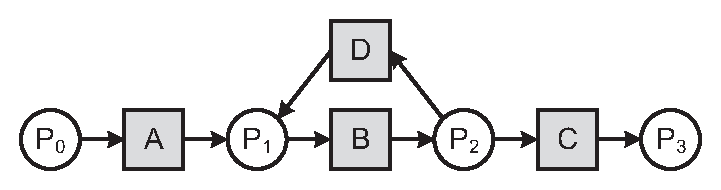
\includegraphics[width=0.45\textwidth]{fig_similarity_1}
% 	\label{fig:similarityExampleA}
% }
% \hspace{0.5cm}
% \subfigure[Model $Q$] {
% 	\centering
% 	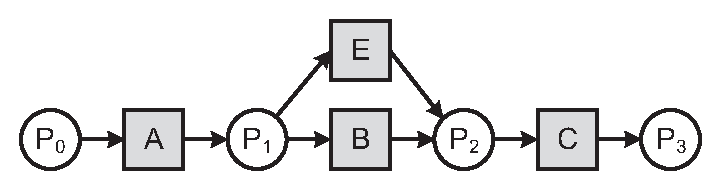
\includegraphics[width=0.45\textwidth]{fig_similarity_2}
% 	\label{fig:similarityExampleB}
% }
% \caption{Example petri nets $P$ and $Q$ for similarity measure\label{fig:similarityExample}}
% \end{figure}

% \begin{table}[htbp]
% \centering
% \tabcaption{Extended relations of the two models in Figure \ref{fig:similarityExample}\label{tab:similarityExample}}
% \subtable[Extended relation matrix of $P$] {
% 	\begin{tabular}{c|c|c|c|c} \hline
% 		Transitions & $A$ & $B$ & $C$ & $D$\\ \hline
% 		$A$
% 			& \multicolumn{1}{>{\columncolor{gray1}}c|}{$\nrightarrow\nleftarrow\nparallel$}
% 			& \multicolumn{1}{>{\columncolor{gray1}}c|}{$\twoheadrightarrow\nleftarrow\nparallel$}
% 			& \multicolumn{1}{>{\columncolor{gray1}}c|}{$\twoheadrightarrow\nleftarrow\nparallel$}
% 			& \multicolumn{1}{>{\columncolor{gray2}}c|}{$\rightharpoonup\nleftarrow\nparallel$}
% 			\\ \hline
% 		$B$
% 			& \multicolumn{1}{>{\columncolor{gray1}}c|}{$\nrightarrow\leftharpoonup\nparallel$}
% 			& \multicolumn{1}{>{\columncolor{gray1}}c|}{$\rightharpoonup\leftharpoonup\nparallel$}
% 			& \multicolumn{1}{>{\columncolor{gray1}}c|}{$\rightharpoonup\nleftarrow\nparallel$}
% 			& \multicolumn{1}{>{\columncolor{gray2}}c|}{$\rightharpoonup\leftharpoonup\nparallel$}
% 			\\ \hline
% 		$C$
% 			& \multicolumn{1}{>{\columncolor{gray1}}c|}{$\nrightarrow\twoheadleftarrow\nparallel$}
% 			& \multicolumn{1}{>{\columncolor{gray1}}c|}{$\nrightarrow\twoheadleftarrow\nparallel$}
% 			& \multicolumn{1}{>{\columncolor{gray1}}c|}{$\nrightarrow\nleftarrow\nparallel$}
% 			& \multicolumn{1}{>{\columncolor{gray2}}c|}{$\nrightarrow\leftharpoonup\nparallel$}
% 			\\ \hline
% 		$D$
% 			& \multicolumn{1}{>{\columncolor{gray2}}c|}{$\nrightarrow\leftharpoonup\nparallel$}
% 			& \multicolumn{1}{>{\columncolor{gray2}}c|}{$\twoheadrightarrow\twoheadleftarrow\nparallel$}
% 			& \multicolumn{1}{>{\columncolor{gray2}}c|}{$\rightharpoonup\nleftarrow\nparallel$}
% 			& \multicolumn{1}{>{\columncolor{gray2}}c|}{$\rightharpoonup\leftharpoonup\nparallel$}
% 			\\ \hline
% 	\end{tabular}
% }
% \subtable[Extend relation matrix of $Q$] {
% 	\begin{tabular}{c|c|c|c|c} \hline
% 		Transitions & $A$ & $B$ & $C$ & $E$\\ \hline
% 		$A$
% 			& \multicolumn{1}{>{\columncolor{gray1}}c|}{$\nrightarrow\nleftarrow\nparallel$}
% 			& \multicolumn{1}{>{\columncolor{gray1}}c|}{$\rightharpoonup\nleftarrow\nparallel$}
% 			& \multicolumn{1}{>{\columncolor{gray1}}c|}{$\twoheadrightarrow\nleftarrow\nparallel$}
% 			& \multicolumn{1}{>{\columncolor{gray3}}c|}{$\rightharpoonup\nleftarrow\nparallel$}
% 			\\ \hline
% 		$B$
% 			& \multicolumn{1}{>{\columncolor{gray1}}c|}{$\nrightarrow\twoheadleftarrow\nparallel$}
% 			& \multicolumn{1}{>{\columncolor{gray1}}c|}{$\nrightarrow\nleftarrow\nparallel$}
% 			& \multicolumn{1}{>{\columncolor{gray1}}c|}{$\twoheadrightarrow\nleftarrow\nparallel$}
% 			& \multicolumn{1}{>{\columncolor{gray3}}c|}{$\nrightarrow\nleftarrow\nparallel$}
% 			\\ \hline
% 		$C$
% 			& \multicolumn{1}{>{\columncolor{gray1}}c|}{$\nrightarrow\twoheadleftarrow\nparallel$}
% 			& \multicolumn{1}{>{\columncolor{gray1}}c|}{$\nrightarrow\leftharpoonup\nparallel$}
% 			& \multicolumn{1}{>{\columncolor{gray1}}c|}{$\nrightarrow\nleftarrow\nparallel$}
% 			& \multicolumn{1}{>{\columncolor{gray3}}c|}{$\nrightarrow\leftharpoonup\nparallel$}
% 			\\ \hline
% 		$E$
% 			& \multicolumn{1}{>{\columncolor{gray3}}c|}{$\nrightarrow\twoheadleftarrow\nparallel$}
% 			& \multicolumn{1}{>{\columncolor{gray3}}c|}{$\nrightarrow\nleftarrow\nparallel$}
% 			& \multicolumn{1}{>{\columncolor{gray3}}c|}{$\twoheadrightarrow\nleftarrow\nparallel$}
% 			& \multicolumn{1}{>{\columncolor{gray3}}c|}{$\nrightarrow\nleftarrow\nparallel$}
% 			\\ \hline
% 	\end{tabular}
% }
% \end{table}

\section{Experimental Evaluation}\label{sec:experiments}
We have implemented an algorithm\footnote{https://github.com/shudiwsh2009/ExRORU} to extract ExRORUs from a process model based on the CPU in jbpt\footnote{https://code.google.com/p/jbpt/}. In this section, we present the experimental evaluation of our algorithm from both effectiveness and efficiency perspectives. We evaluate the effectiveness by comparing it with other algorithms and evaluate the efficiency by applying our algorithm on real-life datasets.

\subsection{Effectiveness Comparison}\label{subsec:effectiveness}
Examples in this section together with the WF-nets in Figure \ref{fig:drawbacks} show the powerful capability of ExRORU to represent the behaviors of a process model.

\paragraph{\textbf{Non-free-choice constructs.}}\label{par:nfc} 
Figure \ref{fig:nfcExampleA} shows a WF-net with non-free-choice constructs \cite{de2003workflow} and Figure \ref{fig:nfcExampleB} shows a similar WF-net that is free choice.

Consider TAR algorithm. The TAR-sets of them are both $\{\langle A,C\rangle, \langle C,D\rangle$, $\langle B,C\rangle, \langle C,E\rangle\}$. However, it is obvious that their behaviors are not the same, since the trace set of the model in Figure \ref{fig:nfcExampleA} is $\{\langle A,C,D\rangle,\langle B,C,E\rangle\}$ while the tract set of the model in Figure \ref{fig:nfcExampleB} is $\{\langle A,C,D\rangle,\langle A,C,E\rangle,\langle B,C,D\rangle,\langle B,C,E\rangle\}$.

Actually, there are only two complete processes in the CPU of the model in Figure \ref{fig:nfcExampleA}, i.e., $[A\{C\}D]$ and $[B\{C\}E]$. Therefore, we have $A\overset{I}{\twoheadrightarrow}D$ and $B\overset{I}{\twoheadrightarrow}E$. On the other hand, there are four complete processes in the CPU of the model in Figure \ref{fig:nfcExampleB}, i.e., $[ACD],[ACE],[BCD],[BCE]$, indicating $A\overset{I}{\rightharpoonup}D$ and $B\overset{I}{\rightharpoonup}E$. Thus, ExRORU can detect the differences between these two models.

\paragraph{\textbf{Multi-relation.}} As noted above, in general multiple relations may exist between two transitions $X$ and $Y$ in a process model. To illustrate, an example WF-net and its CPU are shown in Figure \ref{fig:exampleMultiRelation}. \textit{Transitions $A$ and $D$ can have both causal and concurrent relation between them.} From the unfolding in Figure \ref{fig:multiRelExampleCpu}, we know there are two complete processes, i.e., $[I\{AC,BD\}O]$ and $[I\{A\}E\{D\}O]$. Using ExRORU, we have $A\overset{I}{\rightharpoonup}D$ and $A\Uparrow D$ simultaneously.

\begin{figure}[htbp]
\centering
\subfigure[A WF-net with multi-relation] {
	\centering
	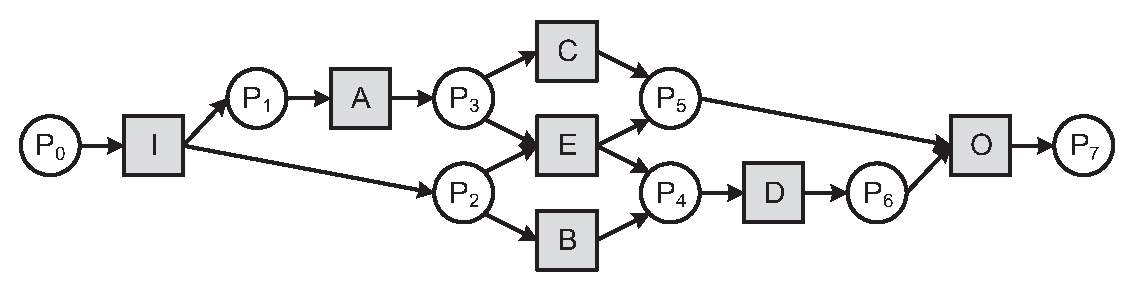
\includegraphics[width=0.46\textwidth]{fig_multi_rel}
	\label{fig:multiRelExample}
}
\subfigure[The CPU of the WF-net in \subref{fig:multiRelExample}] {
	\centering
	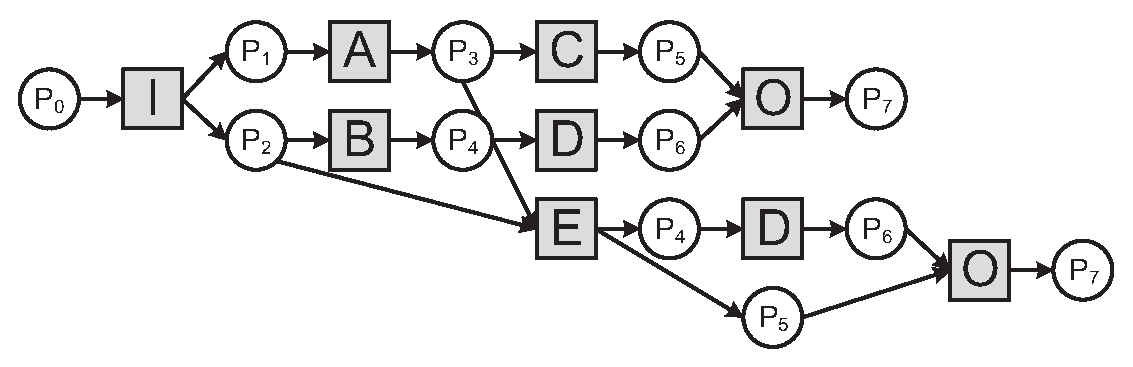
\includegraphics[width=0.46\textwidth]{fig_multi_rel_cpu}
	\label{fig:multiRelExampleCpu}
}
\caption{A WF-net with multi-relation and its CPU\label{fig:exampleMultiRelation}}
\end{figure}

Most algorithms such as BP and TAR cannot recognize the multiple relations in a process model since they categorize each pair of transitions into one type of relation. Hence, they are unable to distinguish between all pairs of process models correctly.

\paragraph{\textbf{Silent transitions}} can also influence the behavior of a model, as mentioned before. In the model pairs of Figures \ref{fig:sdaExampleA}, \ref{fig:sdaExampleB} and \ref{fig:silentExamples}, BP fails to recognize the differences between all four cases because BP doesn't take the adjacency of transitions into consideration, nor can it distinguish \textit{always concurrent} from \textit{sometimes concurrent}. TAR fails in Figures \ref{fig:silentExampleB} and \ref{fig:silentExampleC} due to similar reasons.

On the other hand, ExRORU easily detects the behavioral differences between these model pairs. We have $I\overset{I}{\twoheadrightarrow}O$ in the model of Figure \ref{fig:sdaExampleA} but $I\overset{D}{\twoheadrightarrow}O$ in the model of Figure \ref{fig:sdaExampleB}. In Figure \ref{fig:silentExampleA}, we have $A\overset{D}{\twoheadrightarrow}B$ and $A\overset{I}{\twoheadrightarrow}C$ in the left model but $A\overset{D}{\rightharpoonup}B$ and $A\overset{D}{\twoheadrightarrow}C$ in the right one. And we have $B\Uparrow C$ in the left model but $B\Updownarrow C$ in the right one in both Figures \ref{fig:silentExampleB} and \ref{fig:silentExampleC}.

\begin{figure}[htbp]
\centering
\subfigure[] {
	\begin{minipage}[b]{0.115\textwidth}
		\centering
		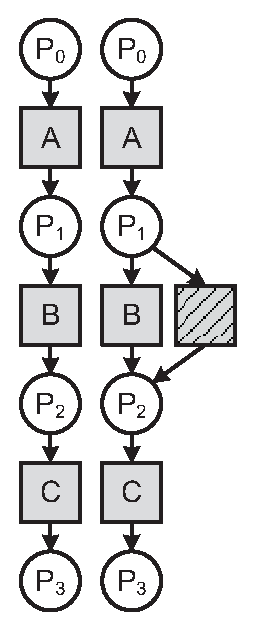
\includegraphics[width=\textwidth]{fig_silent_1}
	\end{minipage}
	\label{fig:silentExampleA}
}
\subfigure[] {
	\begin{minipage}[b]{0.27\textwidth}
		\centering
		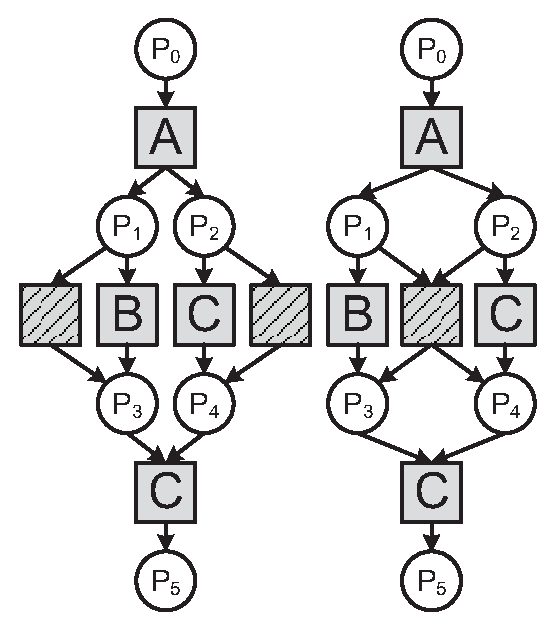
\includegraphics[width=\textwidth]{fig_silent_2}
	\end{minipage}
	\label{fig:silentExampleB}
}
\subfigure[] {
	\begin{minipage}[b]{0.27\textwidth}
		\centering
		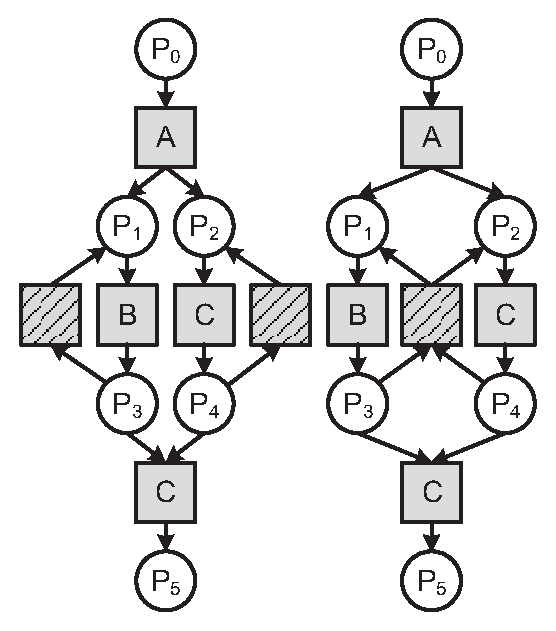
\includegraphics[width=\textwidth]{fig_silent_3}
	\end{minipage}
	\label{fig:silentExampleC}
}
\caption{Example WF-nets with silent transitions that BP and TAR fails in their difference detection\label{fig:silentExamples}}
\end{figure}

\subsection{Efficiency Comparison}\label{subsec:efficiency}
Our dataset contains real-life models from several enterprises such as DG, TC and SAP. The basic features of these model sets are summarized in Table \ref{tab:datasets}.
\\
\begin{table}[htbp]
\centering
\caption{The structural features of real-life process model datasets\label{tab:datasets}}
\scriptsize
\begin{tabular}{|c|r|r|r|r|r|r|r|r|r|r|} \hline
	\multicolumn{1}{|c|}{\multirow{2}{*}{Dataset}} & \multicolumn{1}{c|}{\multirow{2}{*}{Size}} & \multicolumn{3}{|c}{Average} & \multicolumn{3}{|c}{Minimum} & \multicolumn{3}{|c|}{Maximum}\\ \cline{3-11}
	\multicolumn{1}{|c|}{} & \multicolumn{1}{c|}{} & \multicolumn{1}{c|}{\#transitions} & \multicolumn{1}{c|}{\#place} & \multicolumn{1}{c|}{\#arcs} & \multicolumn{1}{c|}{\#transitions} & \multicolumn{1}{c|}{\#place} & \multicolumn{1}{c|}{\#arcs} & \multicolumn{1}{c|}{\#transitions} & \multicolumn{1}{c|}{\#place} & \multicolumn{1}{c|}{\#arcs}\\ \hline
	DG & 94 & 8.56 & 8.89 & 17.78 & 1 & 3 & 3 & 34 & 33 & 70 \\ \hline
	TC & 89 & 11.47 & 10.28 & 22.93 & 6 & 5 & 11 & 28 & 29 & 58 \\ \hline
	SAP & 389 & 4.47 & 7.51 & 11.51 & 1 & 2 & 2 & 21 & 31 & 56 \\ \hline
\end{tabular}
\end{table}

As for comparison, TAR and BP algorithms are based on the relations between tasks as we do while PTS and CFS are based on the abstract trace sets. Therefore, we conduct experiments using ExRORU together with the four above and compare their efficiency. The average time costs on extracting behavioral features of each process model by all the algorithms are shown in Table \ref{tab:efficiency}.
\\
\begin{table}[htbp]
\centering
\caption{Efficiency comparison of all the five algorithms on real-life datasets\label{tab:efficiency}}
	\begin{tabular}{|c|p{1.5cm}<{\centering}|p{1.5cm}<{\centering}|p{1.5cm}<{\centering}|p{1.5cm}<{\centering}|p{1.5cm}<{\centering}|} \hline
		\diagbox{Dataset}{Cost(ms)}{Algo} & TAR & BP & PTS & CFS & ExRORU\\ \hline
		DG & 0.41 & 2.15 & 0.52 & 0.42 & 10.89\\ \hline
		TC & 0.59 & 2.01 & 0.39 & 0.40 & 15.34\\ \hline
		SAP & 0.09 & 0.37 & 0.06 & 0.07 & 1.43\\ \hline
	\end{tabular}
\end{table}

As we can see from the result, ExRORU is the slowest algorithm due to the following reasons. Firstly, models in these datasets are lack of parallel constructs so that the problem of state space explosion may not happen in algorithms utilizing reachability graph or coverability tree such as PTS, CFS and TAR. Secondly, most of the time consumption in similarity measure such as CFS is spent in the similarity computation between the behavioral features of models, which is not considered in our experiment of extracting behavioral features. Finally, considering that ExRORU contains much more details about relations between tasks than other algorithms, the time cost of it is acceptable. To our best knowledge, ExRORU is the only existing algorithm that can handle many complex structures such as silent transitions, non-free-choice constructs and multi-relation, which shows its outstanding effectiveness.

\subsection{Scalability Comparison}\label{subsec:scalability}
We have artificially constructed two sets of process models to test the scalability of five algorithms. The first set contains 11 models with increasing numbers ($5,10,...,55$) of concurrent branches with only one transition on each of them, which we call breadth-scalability dataset. The other one contains 11 models with exactly five concurrent branches but increasing numbers ($1,2,3,...,11$) of sequential transitions on each of them, which we call depth-scalability dataset. The time costs on extracting behavioral features of both datasets are shown in Figure \ref{fig:scalability}. Note that we can only capture the time costs of TAR, PTS and CFS on the first two or three models of both datasets because the problem of state space explosion occurs. The time costs of TAR, PTS and CFS increase extremely fast due to the problem of state space explosion while ExRORU has an acceptable efficiency performance compared to BP.

\begin{figure}[htbp]
\centering
\subfigure[Breadth-scalability dataset] {
	\begin{minipage}[b]{0.46\textwidth}
		\centering
		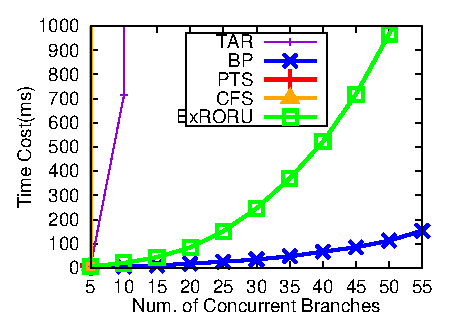
\includegraphics[width=1.0\textwidth]{fig_scalability_breadth}
	\end{minipage}
	\label{fig:scalabilityA}
}
\subfigure[Depth-scalability dataset] {
	\begin{minipage}[b]{0.46\textwidth}
		\centering
		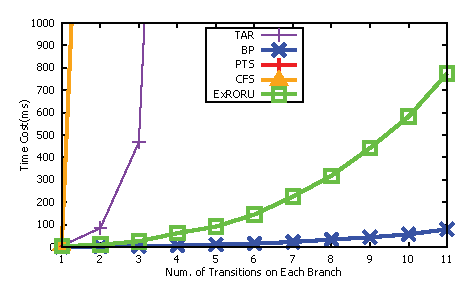
\includegraphics[width=1.0\textwidth]{fig_scalability_depth}
	\end{minipage}
	\label{fig:scalabilityB}
}
\caption[Scalability comparison of five algorithms]{Scalability comparison of the five algorithms on sychesized process models \label{fig:scalability}}
\end{figure}

\section{Conclusion}\label{sec:conclusion}
To better describe the relations between the execution of tasks in a process model, we extend a previous work on refined ordering relations with uncertainty. In this paper, we define three categories of extended relations, which can be further refined into 13 types. With the help of all these 13 kinds of different extended refined ordering relations with uncertainty, subtle behavioral difference between any pair of process models will be detected. We give the computation of our extended relations based on unfolding. Experiments show that our algorithm is the only existing algorithm that can handle many complex structures and has an acceptable time performance.

While our algorithm is not the fastest when compared to other algorithms that rely on the relations between tasks to characterize process models, however it can always uniquely differentiate between any pair of models. Faster implementations will be explored in future work. Furthermore, the main properties of ExRORU will be investigated thoroughly and shown with formal proofs. Finally, we will apply ExRORU on more real-life datasets from different enterprises having process models of various sizes.

\paragraph{\textbf{Acknowledgement.}} The work is supported by National Science Foundation of
China Projects (No. 61472207 \& No. 61325008) and the Special Foundation for Innovation of
Shandong, China (No. 2013CXC30001).

\bibliographystyle{plain}
\bibliography{ref}
\end{document}